\chapter{个人量化管理} % Introduction chapter suppressed from the table of contents


\framebox{%
\begin{minipage}[t]{0.97\columnwidth}\raggedright
我:你们管理层和客户都比较关心项目的进度,项目是否能按时完成?请问你们过去的项目如何?\\开发:我们现在就是走敏捷开发,两周一个迭代。每次迭代前,我们聚一起开会,把所有用户故事按优先级排序,估计这个迭代可以完成哪些任务?然后放在看板的待办事项里。每天我们会做站立会议,监控实际的进展\\我:你们都能按计划在冲刺迭代里把所有任务开发好吗?\\开发想了一下,说:我们也有延误出现,有些模块不能在计划的冲刺里完成。\\我:为什么?\\开发:我们花了很多时间修正系统测试暴露的问题,有一些是因为前面没有把需求分析透导致的返工。\\我:请问你们是怎么估计每个任务应该花多少时间?\\ 开发:我们会一起讨论,然后用敏捷的扑克牌方式,集思广益,估计出来。\\ 我:除了你们每天站立会议监控项目的进展,你们要不要统计一下项目延期的水平是多少?\\开发:其实我们也不算是延误,有些模块不能在本迭代完成,就放在下一个迭代去做。\\ 我:软件开发有一个系数叫每人的生产率,就是开发人员一天能产出多少有效代码?你们有统计吗?\\开发:你说的是否是敏捷开发燃烧图里的速度(Velocity)?我们有画,但发现变化波动很大,所以后面我们也没有再用。\\ 
\strut
\end{minipage}}

\hypertarget{ux5982ux4f55ux964dux4f4eux9879ux76eeux8fdbux5ea6ux504fux5dee}{%
\subsection{如何降低项目进度偏差}\label{ux5982ux4f55ux964dux4f4eux9879ux76eeux8fdbux5ea6ux504fux5dee}}

从以上对话可以看到,敏捷开发不一定能帮助团队按期交付,开发人员也不清楚自己的生产率是多少。要减少项目的延误,首先取决于估算是否准确。但如果只是依赖个人经验、头脑风暴去估计,很可能低估,因为可能没有考虑开发以外的一些因素,比如缺陷问题、需求问题等等。在同一个冲刺里,不能交付所有计划的模块,等同于延误。要做好估算,就需要有数据。数据需要从个人从收集的历史数据作为参考。IT公司是否有注意这方面?我们可以从他们的新员工入职培训探索一下。

\framebox{%
\begin{minipage}[t]{0.97\columnwidth}\raggedright
我:请问你们如何培训新入职的开发人员?\\ 内部培训师:我们会先上一些基础的理论课,培训公司的代码规范、框架和复用的模块。然后进行个人或小组练习,我们会简化一些简单的开发项目里面的某个模块,让他们照着做个小项目,然后我们就会对他们的成果进行反馈,让他们知道自己的开发水平如何,是否掌握了我们所培训的内容。\\ 我:他们会收到什么反馈?\\培训师:理论培训后会有一些选择题考试,会出成绩。我们也会对他们做出来的程序打分。\\我:怎样打分?\\培训师:我们依据评判标准打分,分数从1-5,1最低,5最高。\\我:评判的标准可以说说吗?\\培训师:(想了一下)
依据他们是否掌握了培训内容的重点打分。\\我:你们公司不是已经开始推行量化项目管理,是否应该也配合量化管理,不仅仅靠老师主观判断打分?\\ 培训师:可否举些例子?\\我:例如他们质量方面的缺陷数,如果他们有做单元测试或者评审相关阶段的缺陷排除,项目管理相关所花费的工时,从而可以反算出来编码的效率等客观的量化指标。\strut
\end{minipage}}

\hypertarget{ux4eceux91cfux5316ux57f9ux8badux5f00ux59cb}{%
\subsection{从量化培训开始}\label{ux4eceux91cfux5316ux57f9ux8badux5f00ux59cb}}

从以上对话可以看出很多公司都没有与量化软件开发项目管理相关的培训,这样如何能希望他们在项目中做好量化管理?入职不仅需要培训开发的技巧、怎么写好程序、做好面向对象设计,也应该学到要一直度量自己的开发过程,包括所花的工时,过程中发现的缺陷数等。\\
培训师:在我们新员工培训时,如何可以加入这些量化的元素?\\
我:很简单。首先,在先培训质量相关的技术指标,比如什么叫质量成本,什么叫排除率等,然后做实战练习时,要求他们除了写程序,还需要记录一下所花的工时,自己项目走查时发现的缺陷数,测试的缺陷数,评审所花的时间等等。也要求开发人员除了提交程序以外,提交一个开发计划报告,内容包括实际所花工时,本来预估的工时,过程里发现得缺陷数,在哪一类过程等等。帮助他们一进入公司就培养一些量化度量的习惯,以避免过了试用期,开发的习惯已经养成,后面是很难改变的。\\

\hypertarget{ux4e92ux52a8ux57f9ux8bad}{%
\subsection{互动培训}\label{ux4e92ux52a8ux57f9ux8bad}}

举例:敏捷的小组传球游戏:\\
开头让人员传球,每做完一轮以后再估计下一轮的可以传多少个球。道理一样,让团队可以有据可依,更好地估计下一轮迭代。

本来这个传乒乓球的游戏,目的是让团队参考上一个迭代的数据,估计下一个迭代。但因为每个迭代开发的东西不一样,有些模块是复用的,有些是重新开发的,肯定所花的工作量不一样,所以虽然用以往经验估算下一个迭代概念上没有问题,但实际上可适用的场景很有限。如何可以帮团队做好估算与监控?可以看看我的亲身实验。

\hypertarget{ux4eceux4f30ux7b97ux7b56ux5212ux5230ux76d1ux63a7}{%
\subsection{从估算、策划到监控}\label{ux4eceux4f30ux7b97ux7b56ux5212ux5230ux76d1ux63a7}}

挣值分析(Earned Value EV)是常用的项目监控技巧,
没有项目管理工具也可以简单手动做用挣值分析。Humphrey先生出版了不少书,他都用EV分析来监控进度,他在PSP书中以此为实例,介绍了如何用挣值分析策划与监控。

%\href{文件:PSP_fig7.2.jpg}{350px}

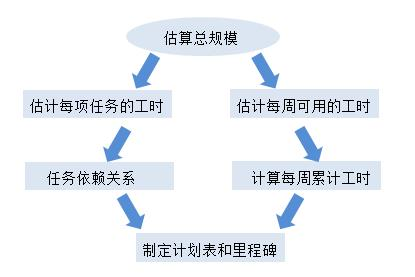
\includegraphics[width=10cm]{PSPfig72.jpg}

下面我也用同样思路来监控本书的进度:\\


今天11月8日,离年底要交书的全部初稿给出版社时间不到两个月,书的内容也完成了超过一半,但剩下的时间因为年底密密麻麻很多评估,而且评估就是早上九点开始到下午五六点结束,只有中间一些空档时间和周末可以自由安排,所以我就用他的思路来策划估算是否能在年底完成要求。
第一步算出现在到年底可以用在写书的时间,按每周估计:

%\url{文件:psp3.jpg}

\includegraphics[width=10cm]{psp3.jpg}

第二步从历史的数据估算剩下的章节,每个章节需要多少小时,写出计划的完成顺序,然后依据原计划可以使用的每周时间,按最佳使用算出每个章节可以在哪周完成,写在表格的右面空白处,从而就可以估算出完成所有章节何时可以完成,如果确实不能到12月底完成,就可能要重新调整、策划,是否有一些章节优先级比较低,暂时不放在第一版。

因觉得单点估算很难定一个点数,便用三点估算法。每一行估计都有三点:最差、最佳、最可能,用
PERT方程式估计预计(Expected) 和 标准差(Sigma)。\\
:(实际顺序可能会有变,以上是已调整版本,原本 MGR 章节是放在后面。。。)

挣值析法所有东西 -- EV, PV, AC
都是用钱来结算(这个例子我们就是用所花工时),例如我们估计了每个章节所需要的工时,利用三点估算计算出每个章节预计的工时,加起来得出预计总工时是80.33工时(用PERT公式计算)。例如第一个章节TDD,预期工时是2.5,除以80.33就得出0.031,我们就用3.1作为TDD的PV(所有任务完成的总PV大概是100)。同样方式算出MGR章节的PV是6.6。(我本来也犯错,以为PV是和产出多少,或页数,成比例,但如用页数作为PV单位的话,就跟其它挣值分析法的系数,如EV,对不上了,导致错误。)得出每一个章节对应的PV后,我们就可以计算累计的PV数:

%\href{文件:psp1.1.jpg}{600px}

\includegraphics[width=10cm]{psp11.jpg}

估计哪一周可以完成哪些章节,得出总体的进度计划。例如第三周累积有66工时,应可完成总共12(=1+4+7)
个章节,因用PERT 三点估算,累积工时95\%范围是(55.8 \textasciitilde{}
62.5)(详见附件)。

%\href{文件:PSP3wksPlanScreenshot_2022-11-26_085813.jpg}{600px}

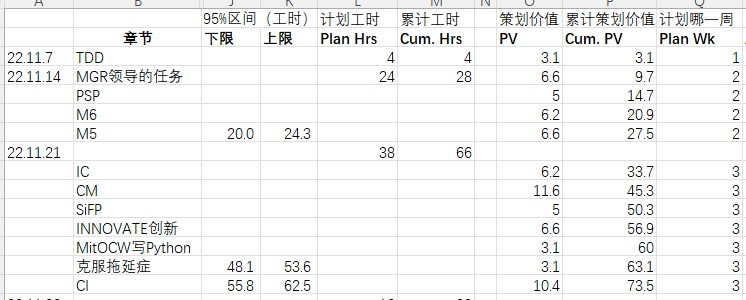
\includegraphics[width=10cm]{PSP3wksPlanScreenshot20221126085813.jpg}

\hypertarget{ux76d1ux63a7}{%
\subsubsection{监控}\label{ux76d1ux63a7}}

按实际完成的情况就可以填右面EV挣值那栋,挣值的算法很简单,必须整个章节完成才算有挣值,不接受部分完成。比如第一周虽然TDD章节已完成九成,但实际是到第二周头才完成,所以第一周的挣值为0。到了第二周才把本来的第一章节完成,所以里面才放上它的PV(=3.1)。监控的好处,好比要准备半年后跑马拉松,开始长距离慢跑LSD锻炼,再进一步做连续马拉松配速训练,每周三天,每次5到15公里,速度是多少?比如平均每公里6:25分钟,有了数字才知道现状与标准的差距,才有动力对自己说现在离比赛不到12周,必须加强锻炼才能赶上。\\
要让项目有更大的机会按期完成,便需要监控,一直可以预计自己离最后交付差距多少?如果按现在的进展要到哪一周才可以完成,应都可以从数字预计出来。但是我们写书也靠灵感,跟写程序类似,可能顺序不一定按本来的执行,怎么办?\\
其实道理也一样,你可以按新的顺序更新一下本来的计划,也把实际的填上。如果你是用简单的Excel表,这个改变可能只花几分钟,很快就能调整好顺序。(例如,本来
现在看到的第二章节,本来计划放在后面才写,但因刚好预客户接触,有灵感,便放在前面写了。)

%\href{文件:PSPend2ndWkEvScreenshot_2022-11-26_091326.jpg}{600px}


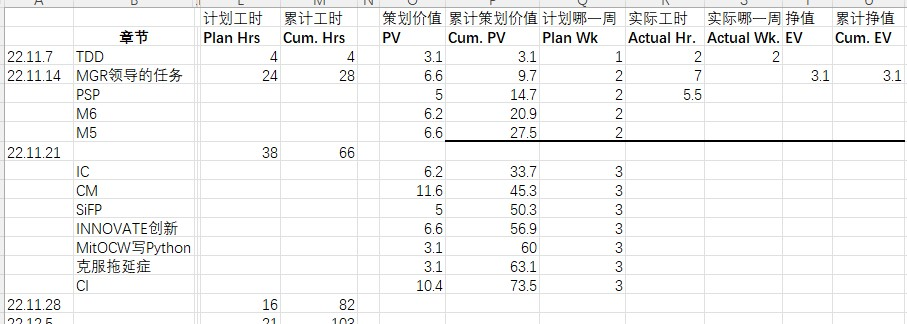
\includegraphics[width=10cm]{PSPend2ndWkEvScreenshot20221126091326.jpg}

要估算任务工时便要依赖以往类似活动的历史记录,如果不是每天记录,过后无法记得住。每周依据个人的习惯,每天记录实际所花小时,然后统计每周累计。但很多人都没有这个习惯,如何养成这个习惯?(详见附件)


\hypertarget{ux603bux7ed3}{%
\subsection{总结}\label{ux603bux7ed3}}

很多软件开发项目延误(或到交付前团队通宵达旦加班)的原因是因为以前没有收集历史数据,导致估计所需人时都很理想。我也有同样问题:从我的挣值分析实例看到,因我是第一次写书,之前也没有养成统计章节所花的实际工时的习惯,所以在11月初做估算时,理想地认为可以最多花一个月完成,但过了3周就发现,实际比本来计划延误很多,原因包括:

\begin{itemize}
\tightlist
\item
  实际可用工时没有想象这么理想,有很多意外事情都要处理。
\item
  低估了完成一章节所需时间:

  \begin{itemize}
  \tightlist
  \item
    例如第一个章节TDD实际所花的工时与估计差不多,原因是这个章节是现有的,只是做了一些调整,所花时间不多;
  \item
    但到第二个章节MGR就不一样了,全部内容都是重新写的,也是从实际的客户现场、场景总结出来,如何与理论结合也很花心思。
  \end{itemize}
\end{itemize}

所以下次当你遇到一些团队项目延误,可以问组长,或者项目经理,如下问题:

\begin{enumerate}
\tightlist
\item
  如何估算项目工期\\
\item
  如何估算每一项任务所需的工时,依据什么?\\
\item
  如何收集实际工作量\\
\item
  如何监控累计到现在的完成情况\\
\item
  有没有统计以往的历史数据?如何用来帮助做好估算?\\
\end{enumerate}

他可能说都有做,当你深入探索时,会发现很多类似我前面挣值分析、监控和估算等问题。

\hypertarget{ux5e94ux8be5ux5982ux4f55ux6539ux5584}{%
\subsection{应该如何改善}\label{ux5e94ux8be5ux5982ux4f55ux6539ux5584}}

软件开发和工业生产不同,工作量数据必须靠个人自己收集,是一个习惯的问题。所以
Humphrey先生在90年代,推出了PSP个体软件过程,教导开发人员如何一步步自己收集数据、自己估算、自己监控,从最基础的记录花多少工时、发现多少缺陷、完成多少代码开始,逐步改善、提升,最终达到管理质量成本,尽量减少缺陷返工。详见附件PSP简介。

也正因为大部分的团队都没有收集数据的良好习惯,没有的PSP的基础,所以就很难要求他们在冲刺回顾时拿出数据,做根因分析,做下一轮的改善,不能从一个定性的管理升为以数据说话、量化管理的状态。反之,当开发人员养成了这习惯,他们就会更清楚知道自己的速度水平和质量水平,不会出现开头说那种情况,对自己的开发质量水平或生产率一无所知,只说已把上级安排的任务尽力做完。\\
有些企业深知量化管理对企业发展很重要,所以在新员工培训时,不仅仅教他们技术技能,也教他开始自己每天记录工时、缺陷数等习惯。
因为新员工入职后,工作习惯就开始养成,后面要改变他们习惯很难。他甚至会觉得既然周边的人都没有这么做,为什么他要统计数据。

\framebox{%
\begin{minipage}[t]{0.97\columnwidth}\raggedright
\textbf{Q\&A}\\
\textbf{资深敏捷顾问}:我大约接近20年前对这个东西比较熟,PSP里边一个包含两个重点:

\begin{enumerate}
\tightlist
\item
  关于个体的估算的内容,这个我看您的文章里边表达的比较充分,
\item
  关于缺陷记录分类统计和根因分析的内容,这一块实际上相当于是cmmi5级里边需要个体配合的地方。我看您几乎没有提到。
\end{enumerate}

我:非常赞同,若要做到本手册后面里提到基于缺陷数据的量化根因分析并改进就要依赖个人记录缺陷与返工工作量,碍于篇幅有限,这里先用人时的估算与监控带出PSP的思路。\\
顾问:我自己也是在某军工航空项目里边用过一次。我们当年计划少跟踪多,大家本来就缺少生产率的概念,所以其实也不知道每天能干什么事,但只要记下来每天干了什么事,然后再往后比照的这个基数做就可以了。无论突然更快了或者更慢了,都需要看看(回顾)到底是为什么。\\
我:您觉得这种方法有用吗?\\
顾问:因为开发是需要创造力的,写新程序其实很难准确估计所需时间,但我后来发现如果估算是由组长负责去做,就能起很大的作用。例如有一次,我看有一个程序员花了一个月时间用java写了某模块,接近一万行代码。虽然我不熟悉Java语言,但觉得代码有点问题。后面我就找另外一个比较资深的组长,三位一起看代码。评审并删除无用的代码,最后剩下不到一百行代码就可以实现了。如果当初我们先做好这模块的估计,就可以避免一个月人时的浪费。所以我建议还是需要估算,但是应该有有经验的技术组长负责。\\
我:很好,你很熟悉敏捷,例如Scrum里用扑克牌方法估算,你觉得怎么样?\\
顾问:我先跟你讲个故事:我参加某冲刺估算会议,它们用扑克牌方法都某功能估算:``数据显示``,其中一位估计是8,另外一位估计是40。为什么会差这么多呢?第一位解释只需要展示数据,确实该工作量不大。但第二位理解就不一样了,包括整个数据的分析、输入和展示等,整个过程工作量确实很大。从这里可以看出,如果没有统一理解需求,就难以估算。所以那次以后,所以需求分析应分成``实体''和``行为'',清晰地写出功能需求,减少误会。\\
我:赞同。Humphrey先生在PSP书里强调,要参考历史数据来做好估算,其实也可适用于敏捷估算。不应但靠人的主观判断。\\
顾问:是的,所以我前面强调必须要有经验的主管去负责估算。估算很重要,但是要程序员自己去估很难。所以PSP二十年前的思路,还能适用于现在的敏捷开发团队,帮助他们做好估算。\\
PSP里强调要评审设计、代码并分析缺陷,当时因为只靠人手,所以会很耗时。现在,我们有类似SONAR的静态扫描工具,就可以像机器人一样,做本来耗时的代码评审工作。但SONAR只能针对一些基本语句问题,针对整个OO设计,我们会建议用我们的CCI工具去扫描(例如,查看有没有类过大等问题),补充SONAR扫描的不足。跟PSP代码评审的思路一样,所有扫描出的问题都必须修正。有些团队觉得问题太多了,只处理掉那些重大的问题,剩下一些可能不会直接影响到功能的问题暂时不处理。我不赞同这思路,这么多的问题其实都是累积出来的,如果从一开始都一直有定期处理清空,就不应该累积大量问题,而且这些问题遗漏下来还是对程序有隐患。\\
我:很赞同,
归根到底还是开发人员缺乏保证质量的意识。最近有个团队也是用工具扫描代码,然后我问他为什么找出的部分问题不处理。他说例如定义某个变量,但是没有用,虽然被扫出是问题,觉得不影响程序的运行就不处理。我解释说,这样就好像放了一个地雷,后面还是会爆炸的,所以还是应该要处理。\strut
\end{minipage}}

PSP
要求评审代码,分析每个发现的缺陷,讨论原因,然后后面改进。所以有些人认为PSP成本太高,只适用于高价值高质量要求的项目里(或作为个人修炼,短暂的时期内使用)\\
有很多自动化开发工具,可以利用它们更好实现PSP的原理,尽量不花太多人的时间,同样可以达到提高软件质量目的。\\
估算很重要,要做好,不仅仅要参考历史数据, 也需要对需求有共同的理解。\\
功能点方法是估算功能需求规模的一种标准,下篇会用些实例介绍如何做功能点估算。

\hypertarget{ux9644ux4ef6}{%
\section{附件}\label{ux9644ux4ef6}}

\hypertarget{ux6323ux503cux5206ux6790ux6cd5earned-value}{%
\subsection{挣值分析法(Earned
Value)}\label{ux6323ux503cux5206ux6790ux6cd5earned-value}}

挣值分析法(Earned
Value),用最简单的例子,来说明挣值分析中PV、EV、与AC的意义。

\begin{description}
\tightlist
\item[]
PV:计划完成多少

AC:完成工作的实际成本是多少?

EV:实际完成了多少工作?
\end{description}

公式:

\begin{description}
\tightlist
\item[]
进度偏差 SV = EV - PV , SPI = EV / PV 完成占计划完成的\%

成本偏差 CV = EV - AC , CPI = EV / AC 完成的价值占实际已花成本的\%
\end{description}

本文实例主要关心进度偏差,所以没有计算 AC

例如:截止到22.11.20 , PV 累加本应是 27.5,EV 只有 3.1

\begin{description}
\tightlist
\item[]
所以 进度偏差 SV = EV - PV = 3.1 - 27.5 = -24.4 工时
\end{description}

用PERT公式估算头三周任务累积工时的95\%区间(工时):\\
不用MonteCarlo模拟,直接把12(=1+4+7)章节任务 的ExpectedValue 加起来\\
计算12步总方差:(方差 = \(Sigma^2\))\\
:总方差 = 每步方差的总和\\
总Sigma(=1.69) \(\sigma\)= 总方差的平方(Sq.Root)

\begin{description}
\item[]
\begin{description}
\tightlist
\item[]
EXCEL 公式为:SQRT(SUM(所有方差范围)) = SQRT(SUM(H3:H15))\\
\end{description}
\end{description}

\begin{description}
\tightlist
\item[]
95\%范围下限(=55.8)

\begin{description}
\tightlist
\item[]
EXCEL 公式为:SUM(所有Expected范围)-2*总Sigma = SUM(F3:F15)-2*I15
\end{description}

95\%范围上限(=62.5)

\begin{description}
\tightlist
\item[]
EXCEL 公式为: SUM(所有Expected范围)+2*总Sigma = SUM(F3:F15)+2*I15
\end{description}
\end{description}

%\href{文件:PSPcalculate3wks95rangeScreenshot_2022-11-26_105325.jpg}{500px}

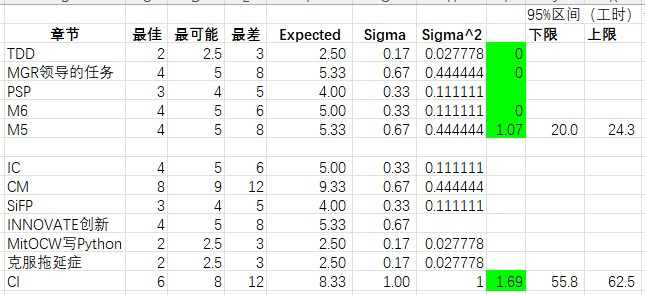
\includegraphics[width=10cm]{PSPcalculate3wks95rangeScreenshot20221126105325.jpg}

\hypertarget{tipsux5982ux4f55ux7b80ux5355ux8bb0ux5f55ux5de5ux65f6}{%
\subsection{Tips:如何简单记录工时}\label{tipsux5982ux4f55ux7b80ux5355ux8bb0ux5f55ux5de5ux65f6}}

如前面``克服拖延症''里提到,每人根据自己的习惯,采用每日ToDoList的方式,然后在开始前,简单记一下时间,结束时也记下时间。然后每日/每周统计每任务总工时:

%\href{文件:Psp手工时间表1.2.jpg}{550px}

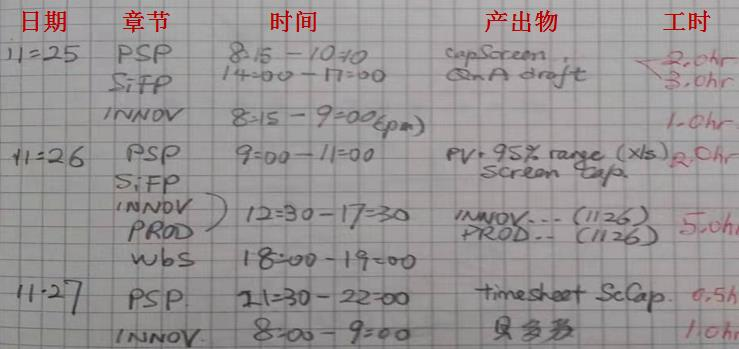
\includegraphics[width=10cm]{Psp手工时间表12.jpg}

(如只是个人,不一定需要项目管理工具;如果是团队,可把自己手工记录上传到项目管理工具,方便团队记录与监控。)

\hypertarget{psp---ux4e2aux4f53ux8f6fux4ef6ux8fc7ux7a0b-personal-software-process-ux7b80ux4ecb}{%
\subsection{PSP - 个体软件过程 Personal Software Process
简介}\label{psp---ux4e2aux4f53ux8f6fux4ef6ux8fc7ux7a0b-personal-software-process-ux7b80ux4ecb}}

\framebox{%
\begin{minipage}[t]{0.97\columnwidth}\raggedright
PSP 的简单介绍\\

\begin{itemize}
\tightlist
\item
  \textbf{PSP0} 基础 - 工时:计划与实际对比; 每阶段引入多少缺陷 ;
  排除了多少缺陷
\item
  \textbf{PSP0.1} 加入 代码行统计 - 计划与实际对比 ; 代码规范
\item
  \textbf{PSP1} 加入 使用 PROBE 方法 做规模估算
\item
  \textbf{PSP2} 加入 设计 与 代码评审的计划与统计
\item
  \textbf{PSP3} Cyclic process - 先做策划与总体设计,然后多轮开发 ;
  有点类似迭代开发。
\end{itemize}\strut
\end{minipage}}

PSP跟CMMI成熟度模型类似,也是按部就班一步步,帮助软件工程师利用度量改进自我的开发过程。

\hypertarget{psp-0.1}{%
\subsubsection{PSP 0.1}\label{psp-0.1}}

第一步PSP先估计写某个模块所需要的时间和实际花的时间,记录所有的缺陷,包括因为需求、设计或者实现引起的问题,记录修复时间,从开始发现问题直到缺陷被解决,提升到PSP0.1策划不仅仅是估计所需时间,加入了规模的概念,本来PSP是用代码行数来估计规模,也可以使用简化功能点方式估计规模大小。\\
在PSP0.1的阶段还没有用规模做策划、估算,只是记录实际的规模,里面包括基本规模,就是在开发之前软件系统本来有多大。也记录删除、改变、增加、复用的规模数等等。最后总的规模数应该是等于基本、新增、删除、复用相加。

\hypertarget{psp1}{%
\subsubsection{PSP1}\label{psp1}}

下一步,PSP1就有规模计划的概念,跟依据0.1的规模定义一样,我们在做开发之前,先估计刚才的所有规模数,并用回归方程估算对应的工作量或者进度,包括偏差的范围。\\
在
PSP0.1增加了一个过程改进建议的环节,依据上一次迭代的数据,发掘下一轮可以完善的改进过程。也加入了编码标准,这个跟我们前面章节提到代码规范的概念相同。所以在PSP0.1,除了计划,也需要有一个叫过程改进经验教训的部分,每一轮都应该有复盘回顾的概念,来提升个人个人的开发过程。

\hypertarget{psp1.1}{%
\subsubsection{PSP1.1}\label{psp1.1}}

PSP1.1基于的PSP1的基础,加入挣值分析法去监控实际的项目进展,加入了PV和累加的PV,计划多少和EV挣值和累计的挣值,反应实际完成多少。从那些系数也可以算出一个叫CPI成本性能指数,来反应完成与计划怎么比较,是否有延误,预计什么时候可以完成。详细可以看用挣值分析法估计写书完成时间的实例。

\hypertarget{psp2}{%
\subsubsection{PSP2}\label{psp2}}

到PSP2就开始增加评审的概念,包括设计评审、代码评审。这些同行评审是很有效的方式,避免缺陷等到出事才暴露、出现问题,因为如果只依赖测试暴露缺陷的话,只是告诉你这个程序跑不通,你还是要看代码才知道问题在哪里,怎么修正?但评审就直接看代码,首先它可以让很多缺陷在评审就发现,就不要等到测试才暴露问题。评审也可以找出一些不一定测得出来的问题,例如有些银行的系统质量要求很高,核心的算法不能有任何错误,他们都会要求核心模块必须走专家评审,因为他们也知道很多一些核心算法的问题不能单靠测试来发现和处理。
也是这个原因,很多公司也会要求代码必须走静态扫描,利用扫描机器人评审代码,预先发现一些明显代码违规的语句问题,弥补单靠人手去评审衡的不足。\\
有了2的基础,2也开始加入缺陷密度的概念,即缺陷数除以模块的规模大小,本来PSP是使用代码行的,我们也可以用功能点取代代码行,因为单看缺陷数无法比较,无论个人自己或者整个团队或者团队之间,所以必须除以规模大小,才可以把系数归一,变成一个项目组之间,人之间可以比较的系数。也引入了排除率的概念,如果我们只是做了评审,但是都是0发现,你的缺陷排除率就是零了,一点效果都没有,所以排除率可以看成是当前评审发现的缺陷数除以当前系统内总共引入的缺陷数,比率越高越好。也有阶段或者过程的排除率,就是这个阶段开始时总共有多少缺陷,然后在这个阶段里我们找出多少,作为分子的一个比例。还有一个就是缺陷排除的速度,按每小时评审的时间找出多少缺陷来判断评审中,可以找出缺陷的速度有多快,评审的效率有多高。

评审质量是PSP2.1 的概念,2.1
也增加质量成本(COQ)概念,与前面敏捷回顾篇里强调软件开发缺陷越后发现,返工量会几何式上升的思路一致。

\hypertarget{psp3}{%
\subsubsection{PSP3}\label{psp3}}

接近敏捷迭代的思路,把程序分成不超于几百行的模块,然后把模块按优先级分到不同的迭代
,但还需要有需求与设计。敏捷增加了精益的思路,因为需求可能会有变,所以可以暂时不做后面迭代的估算,只先针对当前的迭代去做策划、估算。
敏捷里面的迭代回顾跟PSP的回顾如出一辙。\\
大家可以参考PSP书里面的教材和练习,比如在书中要求学员自己编写程序,自己记录时间。虽然现在开发语言统计方法跟90年代有差异,但原理还是共通的。如果对新员工难以安排学校式的一周课程,也可以考虑用自学的形式,按要求去记录学习、写报告。

\framebox{%
\begin{minipage}[t]{0.97\columnwidth}\raggedright
学PSP,培养好习惯
所以编程人员可以用PSP的原则,要他们记录。因为现在是写程序,不是玩游戏,所以更贴近实际。也要求后面的程序,让他分析自己的返工、质量成本、缺陷排除等,让后面项目团队回顾时有真实数据做分析。

例如在新员工培训时,
在练习中,要求他们有编码规范的概念,按照公司的规范参考来写程序,在每一次做开发之前,都先简单计划一下时间和预估缺陷数。开发完后,记录实际的时间与缺陷数,因为虽然不仅仅是写一个程序,是一个系列,在做下一次开发时,可以参考以往练习的数据来更好估计,会看到自己的估计越来越准。\strut
\end{minipage}}

\hypertarget{references}{%
\section{References}\label{references}}

1. Humphrey, Watts S.: "A Discipline for Software Engineering"\\
2. Humphrey, Watts S.: "PSP: A Self-Improvement Process for Software
Engineers" (2005)\\


